\let\negmedspace\undefined
\let\negthickspace\undefined
\documentclass[journal,12pt,twocolumn]{IEEEtran}
%\documentclass[conference]{IEEEtran}
%\IEEEoverridecommandlockouts
% The preceding line is only needed to identify funding in the first footnote. If that is unneeded, please comment it out.
\usepackage{svg}
\usepackage{tikz}
\usepackage{cite}
\usepackage{amsmath,amssymb,amsfonts,amsthm}
\usepackage{algorithmic}
\usepackage{float}
\usepackage{graphicx}
\usepackage{subcaption}
\usepackage{xcolor}
\usepackage{txfonts}
\usepackage{listings}
\usepackage{enumitem}
\usepackage{mathtools}
\usepackage{gensymb}
\usepackage[breaklinks=true]{hyperref}
\usepackage{tkz-euclide} % loads  TikZ and tkz-base
\usepackage{listings}
\usetikzlibrary{positioning}
%
%\usepackage{setspace}
%\usepackage{gensymb}
%\doublespacing
%\singlespacing

%\usepackage{graphicx}
%\usepackage{amssymb}
%\usepackage{relsize}
%\usepackage[cmex10]{amsmath}
%\usepackage{amsthm}
%\interdisplaylinepenalty=2500
%\savesymbol{iint}
%\usepackage{txfonts}
%\restoresymbol{TXF}{iint}
%\usepackage{wasysym}
%\usepackage{amsthm}
%\usepackage{iithtlc}
%\usepackage{mathrsfs}
%\usepackage{txfonts}
%\usepackage{stfloats}
%\usepackage{bm}
%\usepackage{cite}
%\usepackage{cases}
%\usepackage{subfig}
%\usepackage{xtab}
%\usepackage{longtable}
%\usepackage{multirow}
%\usepackage{algorithm}
%\usepackage{algpseudocode}
%\usepackage{enumitem}
%\usepackage{mathtools}
%\usepackage{tikz}
%\usepackage{circuitikz}
%\usepackage{verbatim}
%\usepackage{tfrupee}
%\usepackage{stmaryrd}
%\usetkzobj{all}
%    \usepackage{color}                                            %%
%    \usepackage{array}                                            %%
%    \usepackage{longtable}                                        %%
%    \usepackage{calc}                                             %%
%    \usepackage{multirow}                                         %%
%    \usepackage{hhline}                                           %%
%    \usepackage{ifthen}                                           %%
  %optionally (for landscape tables embedded in another document): %%
%    \usepackage{lscape}     
%\usepackage{multicol}
%\usepackage{chngcntr}
%\usepackage{enumerate}

%\usepackage{wasysym}
%\newcounter{MYtempeqncnt}
\DeclareMathOperator*{\Res}{Res}
%\renewcommand{\baselinestretch}{2}
\renewcommand\thesection{\arabic{section}}
\renewcommand\thesubsection{\thesection.\arabic{subsection}}
\renewcommand\thesubsubsection{\thesubsection.\arabic{subsubsection}}

\renewcommand\thesectiondis{\arabic{section}}
\renewcommand\thesubsectiondis{\thesectiondis.\arabic{subsection}}
\renewcommand\thesubsubsectiondis{\thesubsectiondis.\arabic{subsubsection}}

% correct bad hyphenation here
\hyphenation{op-tical net-works semi-conduc-tor}
\def\inputGnumericTable{}                                 %%
\newcommand{\permcomb}[4][0mu]{{{}^{#3}\mkern#1#2_{#4}}}
\newcommand{\comb}[1][-1mu]{\permcomb[#1]{C}}
\lstset{
%language=C,
frame=single, 
breaklines=true,
columns=fullflexible
}
%\lstset{
%language=tex,
%frame=single, 
%breaklines=true
%}

\begin{document}
%


\newtheorem{theorem}{Theorem}[section]
\newtheorem{problem}{Problem}
\newtheorem{proposition}{Proposition}[section]
\newtheorem{lemma}{Lemma}[section]
\newtheorem{corollary}[theorem]{Corollary}
\newtheorem{example}{Example}[section]
\newtheorem{definition}[problem]{Definition}
%\newtheorem{thm}{Theorem}[section] 
%\newtheorem{defn}[thm]{Definition}
%\newtheorem{algorithm}{Algorithm}[section]
%\newtheorem{cor}{Corollary}
\newcommand{\BEQA}{\begin{eqnarray}}
		\newcommand{\EEQA}{\end{eqnarray}}
\newcommand{\define}{\stackrel{\triangle}{=}}

\bibliographystyle{IEEEtran}
%\bibliographystyle{ieeetr}


\providecommand{\mbf}{\mathbf}
\providecommand{\pr}[1]{\ensuremath{\Pr\left(#1\right)}}
\providecommand{\qfunc}[1]{\ensuremath{Q\left(#1\right)}}
\providecommand{\sbrak}[1]{\ensuremath{{}\left[#1\right]}}
\providecommand{\lsbrak}[1]{\ensuremath{{}\left[#1\right.}}
\providecommand{\rsbrak}[1]{\ensuremath{{}\left.#1\right]}}
\providecommand{\brak}[1]{\ensuremath{\left(#1\right)}}
\providecommand{\lbrak}[1]{\ensuremath{\left(#1\right.}}
\providecommand{\rbrak}[1]{\ensuremath{\left.#1\right)}}
\providecommand{\cbrak}[1]{\ensuremath{\left\{#1\right\}}}
\providecommand{\lcbrak}[1]{\ensuremath{\left\{#1\right.}}
\providecommand{\rcbrak}[1]{\ensuremath{\left.#1\right\}}}
\theoremstyle{remark}
\newtheorem{rem}{Remark}
\newcommand{\sgn}{\mathop{\mathrm{sgn}}}
\providecommand{\abs}[1]{\(left\)vert#1\(right\)vert}
\providecommand{\res}[1]{\Res\displaylimits_{#1}}
\providecommand{\norm}[1]{\(left\)lVert#1\(right\)rVert}
%\providecommand{\norm}[1]{\lVert#1\rVert}
\providecommand{\mtx}[1]{\mathbf{#1}}
\providecommand{\mean}[1]{E\(left\)[ #1 \(right\)]}
\providecommand{\fourier}{\overset{\mathcal{F}}{ \rightleftharpoons}}
%\providecommand{\hilbert}{\overset{\mathcal{H}}{ \rightleftharpoons}}
\providecommand{\system}{\overset{\mathcal{H}}{ \longleftrightarrow}}
%\newcommand{\solution}[2]{\textbf{Solution:}{#1}}
\newcommand{\solution}{\noindent \textbf{Solution: }}
\newcommand{\cosec}{\,\text{cosec}\,}
\providecommand{\dec}[2]{\ensuremath{\overset{#1}{\underset{#2}{\gtrless}}}}
\newcommand{\myvec}[1]{\ensuremath{\begin{pmatrix}#1\end{pmatrix}}}
\newcommand{\mydet}[1]{\ensuremath{\begin{vmatrix}#1\end{vmatrix}}}

\let\vec\mathbf


\vspace{3cm}

\title{
	%	\logo{
	Software Assignment
 
	\Large AI1110: Probability and Random Variables
 
	\Large Indian Institute of Technology, Hyderabad
	%	}
}
\author{
	CS22BTECH11001
	
	Aayush Adlakha
 
	18 May, 2023
	% <-this % stops a space
}






\maketitle

\newpage


\bigskip


\section{Introduction}
In this project, we have developed a Python-based music player using the Pygame library. The music player allows users to play, pause, and navigate through a collection of songs. Additionally, we have included a feature to convert videos to audio files using the MoviePy library.

\section{Random Permutaion}
Numpy library has been used to create a list having values from 0 to 19, when looping through this list, if we reach the end a random permutation is again appended so that we can shuffle the files forever

\section{Music Player}
The music player provides a user-friendly interface for playing and managing songs. It offers the following functionalities:

\begin{itemize}
  \item Play: Clicking the "Play" button starts playing the currently selected song.
  \item Pause: Clicking the "Pause" button pauses the currently playing song.
  \item Next: Clicking the "Next" button plays the next song in the playlist.
  \item Previous: Clicking the "Previous" button plays the previous song in the playlist.
  \item Currently Playing: The music player displays the name of the currently playing song.
\end{itemize}

The music player utilizes the Pygame library to load and play audio files. It keeps track of the playlist using a list of song filenames. The user can navigate through the playlist and control playback using the provided buttons.

\section{Video to Audio Conversion}
The project also includes a video to audio conversion feature. It allows users to convert video files to audio files for easy playback or other purposes. The conversion is done using the MoviePy library.

The video to audio conversion works as follows:

\begin{itemize}
  \item The program scans the project folder for video files.
  \item It identifies video files based on their file extension (e.g., ".mp4").
  \item For each video file found, the program extracts the audio from the video using the MoviePy library.
  \item The extracted audio is saved as an audio file with the same name as the original video file but with the ".mp3" extension.
\end{itemize}

This feature allows users to convert their video files into audio files, which can be useful for various purposes, such as creating audio podcasts or extracting audio tracks from videos.

The code can be found at,
\begin{lstlisting}
    https://github.com/Ad-Aayush/Audio-Shuffle
\end{lstlisting}
\section{Conclusion}
The Python music player project provides a user-friendly interface for playing and managing songs. It allows users to easily control playback and navigate through their song collection. Additionally, the project includes functionalities of the Numpy library to shuffle through the playlist by creating random permutations conversion feature, which enables users to extract audio from video files.


\begin{figure}[h]
    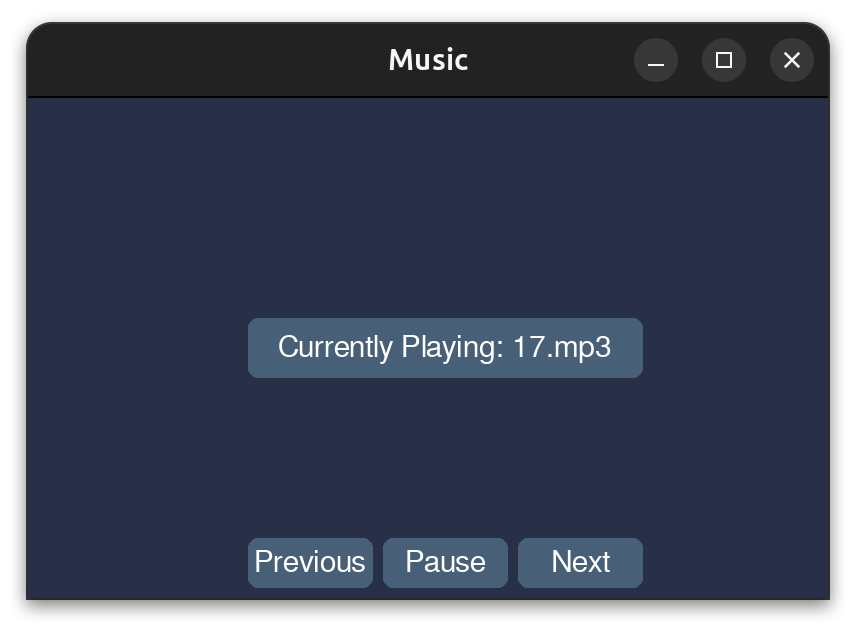
\includegraphics[width = \columnwidth]{figs/1.png}
    \centering
    \caption{Music Player}
    \label{fig:1}
\end{figure}
\begin{figure}[h]
    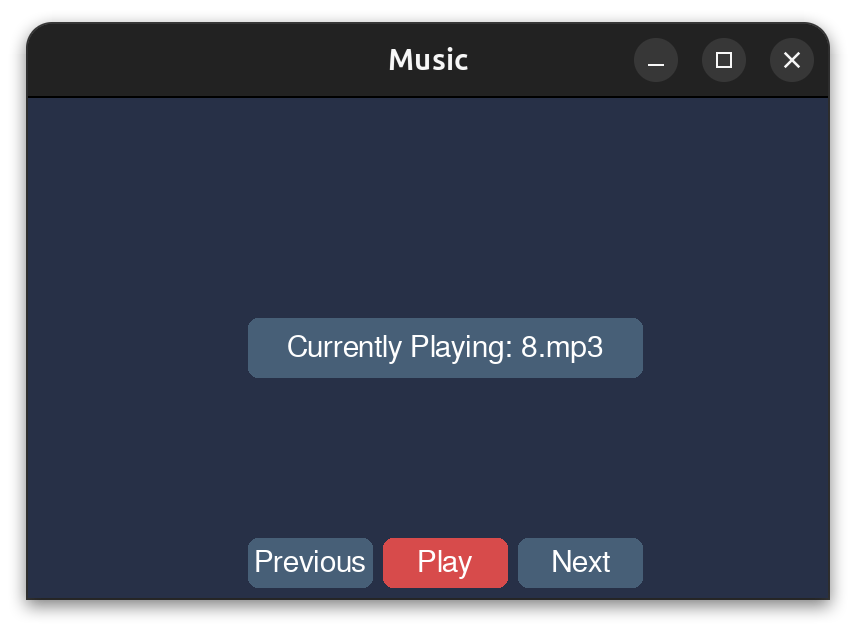
\includegraphics[width = \columnwidth]{figs/2.png}
    \centering
    \caption{Pause/Play button}
    \label{fig:2}
\end{figure}
\end{document}
